\documentclass[crop,tikz,multi=my]{standalone}

\usetikzlibrary{decorations.pathreplacing,positioning,calc,intersections,3d,shapes.geometric,math}

\begin{document}

\newcommand{\SimpGraph}[4]{
	\foreach \x in {1,...,#1} {
		\coordinate (#3\x) at ($#2 + (90-\x*360/#1+180/#1:#4)$);
		\filldraw[black] (#3\x) circle (1pt);}
	\foreach \x in {1,...,#1} {
		\foreach \y in {\x,...,#1} {
			\draw[black] (#3\x) -- (#3\y);}}
	}
\newcommand{\SimpGraphEmpty}[3]{
	\foreach \x in {1,...,#1} {
		\coordinate (#3\x) at ($#2 + (90-\x*360/#1+180/#1:1)$);}
	}
\newcommand{\SimpCoords}{
	\SimpGraphEmpty{3}{(0,0-2)}{S} \SimpGraphEmpty{3}{(3,0-2.5)}{T} \SimpGraphEmpty{3}{(1.5,2-2.5)}{U}
	\path (S3)--(T3) coordinate[midway] (023);
	\path (U3)--(T3) coordinate[near start] (123); % needs shifting?
	\path (S1)--(T1) coordinate[midway] (024);
	\path (U1)--(U3) coordinate[midway] (134);
	
	\path (S1)--(U1) coordinate[near end] (014); % needs shifting?
	\path (S2)--(U2) coordinate[very near end] (015);
	\path (S2)--(T2) coordinate[midway] (025);
	\path (U3)--(U2) coordinate[near end] (135);
	}
	
	\begin{my}
		\begin{tikzpicture}
			\SimpGraph{2}{(0,0-2)}{S}{1}
			\node[right] at (S1) {02}; \node[left] at (S2) {01};
		\end{tikzpicture}
	\end{my}
	
	\begin{my}
		\begin{tikzpicture}
			\SimpGraph{3}{(0,0-2)}{0}{1} \SimpGraph{3}{(3,0-2.5)}{2}{1} \SimpGraph{3}{(1.5,2-2.5)}{1}{1}
			\foreach \x in {1,2,3} {\foreach \y in {0,1} {\foreach \z in {1,2} {\draw[blue] (\y\x) -- (\z\x);}}}
			\foreach \x in {0,1,2} {\foreach \y[count=\i from 3] in {3,1,2} {\node[above] at (\x\y) {\x\i};}}
		\end{tikzpicture}
	\end{my}
	
	\begin{my}
		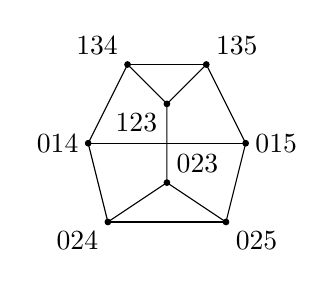
\begin{tikzpicture}
			\coordinate (123) at (0,0);
			\coordinate (023) at (0,-1);
			\coordinate (134) at (-0.5,0.5);
			\coordinate (135) at (0.5,0.5);
			\coordinate (015) at (1,-0.5);
			\coordinate (014) at (-1,-0.5);
			\coordinate (025) at (0.75,-1.5);
			\coordinate (024) at (-0.75,-1.5);
			\node[below left] at (123) {123};
			\node[above right] at (023) {023};
			\node[above left] at (134) {134};
			\node[above right] at (135) {135};
			\node[right] at (015) {015};
			\node[left] at (014) {014};
			\node[below right] at (025) {025};
			\node[below left] at (024) {024};
			\foreach \x in {123,023,134,135,015,014,025,024} {\filldraw (\x) circle (1pt);}
			
			\draw (123) -- (023) -- coordinate[midway] (0234) (024) -- (014) -- (134) -- coordinate[midway] (1234) cycle;
			\draw (123) -- (135) -- coordinate[near end] (0135) (015) -- coordinate[midway] (0125) (025) -- (023);
			\draw (135) -- coordinate[near start] (1345) (134);
			\draw (014) -- (015);
			\draw (024) -- coordinate[near end] (0245) (025);
		\end{tikzpicture}
	\end{my}
	
	\begin{my}
	\begin{tikzpicture}
		\matrix[row sep=0em, column sep=1em, every cell/.style={scale=0.7}]{
		% S=0, T=2, U=1, 1->4, 2->5, 3->3
			\SimpCoords
			\foreach \x in {1,2,3} {\draw[black] (S\x) -- (U\x);}
			\foreach \x in {S,U} {\draw[black] (\x1) -- (\x2) -- (\x3) -- cycle;}
			\filldraw[blue,opacity=0.3] (134) node[above,black,opacity=1] {134} --(135) node[left,black,opacity=1] {135} --(015) node[below,black,opacity=1] {015} --(014) node[right,black,opacity=1] {014} --cycle;
			&
			\SimpCoords
			\foreach \x in {1,3} {\draw[black] (S\x)-- (T\x)-- (U\x)-- cycle;}
			\foreach \x in {S,T,U} {\draw[black] (\x1)--(\x3);}
			\filldraw[blue,opacity=0.3] (134) node[above,black,opacity=1] {134} --(123) node[left,black,opacity=1] {123} --(023) node[below left,black,opacity=1] {023} --(024) node[below right,black,opacity=1] {024} --(014) node[right,black,opacity=1] {014} --cycle;
			&
			\SimpCoords
			\foreach \x in {1,2,3} {\draw[black] (U\x)--(T\x);}
			\foreach \x in {U,T} {\draw[black] (\x1)--(\x2)--(\x3)--cycle;}
			\filldraw[blue,opacity=0.3] (134) node[above,black,opacity=1] {134} --(135) node[below,black,opacity=1] {135} --(123) node[left,black,opacity=1] {123} --cycle;
			\\
			\SimpCoords
			\foreach \x in {1,2} {\draw[black] (S\x)--(T\x)--(U\x)--cycle;}
			\foreach \x in {S,T,U} {\draw[black] (\x1)--(\x2);}
			\filldraw[blue,opacity=0.3] (015) node[left,black,opacity=1] {015} --(025) node[below,black,opacity=1] {025} --(024) node[right,black,opacity=1] {024} --(014) node[above,black,opacity=1] {014} --cycle;
			&
			\SimpCoords
			\foreach \x in {1,2,3} {\draw[black] (S\x)--(T\x);}
			\foreach \x in {S,T} {\draw[black] (\x1)--(\x2)--(\x3)--cycle;}
			\filldraw[blue,opacity=0.3] (023) node[left,black,opacity=1] {023} --(024) node[above right,black,opacity=1] {024} --(025) node[below,black,opacity=1] {025} --cycle;
			&
			\SimpCoords
			\foreach \x in {3,2} {\draw[black] (S\x)--(T\x)--(U\x)--cycle;}
			\foreach \x in {S,T,U} {\draw[black] (\x3)--(\x2);}
			\filldraw[blue,opacity=0.3] (023) node[left,black,opacity=1] {023} --(025) node[below,black,opacity=1] {025} --(015) node[above right,black,opacity=1] {015} --(135) node[above right,black,opacity=1] {135} --(123) node[left,black,opacity=1] {123} --cycle;
		\\};
	\end{tikzpicture}
	\end{my}
	
	\begin{my}
	\begin{tikzpicture}
		\matrix[row sep=0em, column sep=1em, every cell/.style={scale=0.7}]{
		% S=0, T=2, U=1, 1->4, 2->5, 3->3
			\SimpCoords
			\foreach \x in {1,2,3} {\draw[black] (S\x) -- (U\x);}
			\foreach \x in {S,U} {\draw[black] (\x1) -- (\x2) -- (\x3) -- cycle;}
			\foreach \x[count=\j from 3] in {3,1,2} {\foreach \y[count=\i from 0] in {S,U} {\node[above] at (\y\x) {\i\j};}}
			&
			\SimpCoords
			\foreach \x in {1,3} {\draw[black] (S\x)-- (T\x)-- (U\x)-- cycle;}
			\foreach \x in {S,T,U} {\draw[black] (\x1)--(\x3);}
			\foreach \x[count=\j from 3] in {3,1} {\foreach \y[count=\i from 0] in {S,U,T} {\node[above] at (\y\x) {\i\j};}}
			&
			\SimpCoords
			\foreach \x in {1,2,3} {\draw[black] (U\x)--(T\x);}
			\foreach \x in {U,T} {\draw[black] (\x1)--(\x2)--(\x3)--cycle;}
			\foreach \x[count=\j from 3] in {3,1,2} {\foreach \y[count=\i from 1] in {U,T} {\node[above] at (\y\x) {\i\j};}}
			\\
			\SimpCoords
			\foreach \x in {1,2} {\draw[black] (S\x)--(T\x)--(U\x)--cycle;}
			\foreach \x in {S,T,U} {\draw[black] (\x1)--(\x2);}
			\foreach \x[count=\j from 4] in {1,2} {\foreach \y[count=\i from 0] in {S,U,T} {\node[above] at (\y\x) {\i\j};}}
			&
			\SimpCoords
			\foreach \x in {1,2,3} {\draw[black] (S\x)--(T\x);}
			\foreach \x in {S,T} {\draw[black] (\x1)--(\x2)--(\x3)--cycle;}
			\foreach \x[count=\j from 3] in {3,1,2} {\foreach \y/\i in {S/0,T/2} {\node[above] at (\y\x) {\i\j};}}
			&
			\SimpCoords
			\foreach \x in {3,2} {\draw[black] (S\x)--(T\x)--(U\x)--cycle;}
			\foreach \x in {S,T,U} {\draw[black] (\x3)--(\x2);}
			\foreach \x/\j in {3/3,2/5} {\foreach \y[count=\i from 0] in {S,U,T} {\node[above] at (\y\x) {\i\j};}}
		\\};
	\end{tikzpicture}
	\end{my}
	
\end{document}